\section{Wstep teoretyczny} \label{theory}
W~kolejnych podrozdziałach opisane są krótko podstawy teoretyczne dotyczące uczenia maszynowego, wykorzystanych algorytmów oraz~użytych metod optymalizacji.
\subsection{Formalny opis uczenia maszynowego}
Uczenie maszynowe okreslane jest jako jedna z~galezi sztucznej inteligencji \cite{dnn1}. Formalną definicję podał Tom Mitchell, która~brzmi następująco: ,,Mówimy, że~maszyna uczy się zadania $T$ w~oparciu o~doświadczenie $E$ i~miarę jakości $P$, jeśli wraz z~przyrostem doświadczenia $E$ poprawia się jakość wykonywanego zadania $T$ mierzona przez~miarę $P$.''\cite{mitchel} Przykładowo można wymienić trójkę $T$, $E$, $P$ jako diagnozowanie pacjenta na~podstawie symptomów, dotychczasowe  liczba wykonanych przez~maszynę diagnoz (poprawnie lub~nie),  poprawność diagnozowania na~podstawie do~tej pory niespotkanych przypadków. Powyższe przykłady można mnożyć. Zapis formalny (na podstawie \cite{formal2}) w~przypadku algorytmów przedstawionych w~niniejszej pracy możemy przedstawić następująco:
\begin{itemize}
\item $x$ - dane wejściowe algorytmu
\item $y$ - wyjście algorytmu
\item $f$ - funkcja modelowana
\item $g$ - funkcja modelująca.
\end{itemize}
Ogólnie możemy powiedzieć, że~zadaniem algorytmu jest znalezienie takiej funkcji $g$, która~jak~w~najlepszy stopniu przybliża funkcję $f$. Odnosząc to do~przykładu rozpoznawania chorób, możemy powiedzieć, że~modelowaną funkcją jest odwzorowanie symptomów na diagnozę. Uczenie wg danego algorytmu przeprowadza się na~podstawie danych:
\begin{equation}
d = (x_1,y_1), (x_2, y_2), ..., (x_n, y_n).
\end{equation}
Każda para $(x_i, y_i)$ stanowi jeden rekord danych lub~też jeden przykład podawany do~algorytmu, gdzie $x_i$ jest wektorem cech lub też atrybutów danego rekordu, natomiast $y_i$ jest odpowiedzią dla danego $x_i$. W~odniesieniu do~przykładu z~rozpoznawaniem chorób na~podstawie symptomów, jednym rekordem jest konkretny zestaw symptomów ($x_i$) wraz z~diagnozą ($y_i$). W~zależności od~tego, czy~$y_i$ przyjmuje wartości ciągłe czy~dyskretne, mamy do~czynienia z~wykorzystaniem uczenia maszynowego w~problemie kolejno regresji lub~klasyfikacji. W~najbardziej podstawowym przypadku, posiadane dane dzieli się na~dwa zbiory. Jeden z~nich określany jest zbiorem uczącym, a~drugi testującym. Podział dokonywany jest, aby oceniać model na innych danych niż na których został on nauczony. Związane jest to z problemem przeuczenia opisanym w rozdziale \ref{overfitting_section}. W~celu określenia wydajności algorytmu zazwyczaj używa się błędu średniokwadratowego, który~wyraża się wzorem:
% MSE: https://medium.com/human-in-a-machine-world/mae-and-rmse-which-metric-is-better-e60ac3bde13d
\begin{equation}
\frac{1}{n} \sum_{j=1}^{n}(y_j - \hat{y}_j), 
\end{equation}
przy czym $\hat{y}_j$ oznacza odpowiedź stworzonego predykatora dla atrybutów przykładu $i$.
W~kolejnych podrozdziałach autor korzysta również z~określenia niestabilny algorytm uczenia maszynowego. Mamy z~takim do~czynienia, gdy mała zmiana w~danych wejściowych może spowodować dużą zmianę w~predykcjach generowanych przez~algorytm\cite{ensemble}.
%W tej pracy wszystkie metody optymalizacji były analizowane pod kątem problemu klasyfikacji lecz naturalne jest ich użycie w przypadku problemu regresji.

\subsection{Wykorzystane algorytmy}
W~tym podrozdziale opisane są kolejne algorytmy, które~wykorzystywane były w~pracy.
\subsubsection{Drzewo decyzyjne}
%www.cs.princeton.edu/courses/archive/spr07/cos424/papers/mitchell-dectrees.pdf
% scikit-learn uses an optimised version of the CART algorithm.
Drzewo decyzyjne jest algorytmem uczenia maszynowego, który~może posłużyć w~celu rozwiązania problemu klasyfikacji oraz~regresji. Funkcja, która~jest modelowana przez~algorytm przedstawiana jest w~formie drzewa matematycznego. Jest to jedna z~najpopularniejszych metod, która~znalazła swoje wykorzystanie w~diagnozowaniu chorób czy~ocenie ryzyka kredytowego klientów banków\cite{mitchel}. Zaletami tego podejścia jest między innymi  prostota oraz~łatwość interpretacji. Dużą wadą drzew decyzyjnych jest fakt, iż~stworzenia optymalnego drzewa decyzyjnego nie należy do problemów rozwiązywalnych w czasie wielomianowym. W~praktyce tworzenie drzewa oparte jest na~metodach heurystycznych\cite{dtscikit}. Na~rysunku \ref{dt1image} przedstawione zostało przykładowe drzewo, które~mogłoby posłuży do~klasyfikacji danych o~trzech atrybutach na~trzy klasy. Można stwierdzić, że~drzewo decyzyjne jest tzw. białą skrzynką (\textit{whitebox}), ponieważ~łatwo można zauważyć na~jakiej podstawie podjęta została decyzja przyporządkowania do~danej klasy.

\begin{figure}[ht!]
\centering
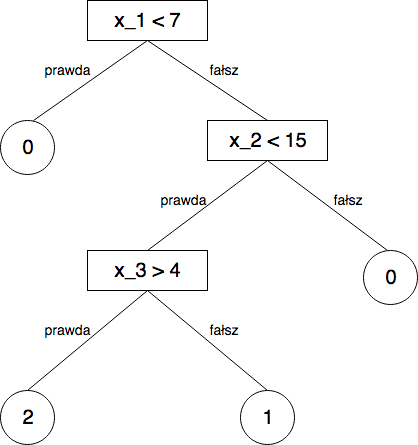
\includegraphics[scale=0.6]{res/dt1.png}
\caption[Caption for LOF]{Przykład drzewa decyzyjnego.\label{dt1image}}
\end{figure} 

\paragraph{Tworzenie drzewa decyzyjnego}\mbox{}\\
%ftp://ftp.boulder.ibm.com/software/analytics/spss/support/Stats/Docs/Statistics/Algorithms/14.0/TREE-CART.pdf
Istnieją różne sposoby na~stworzenie drzewa klasyfikacyjnego. Jednym z~nich jest algorytm CART -\textit{Classification  and  Regression  Trees}, który~był wykorzystany w~tej pracy i~jest opisany w~tym paragrafie. Ideą tego podejścia jest dzielenie danych wejściowych na~rozłączne i~dopełniające się podzbiory w~taki sposób, aby~zbiory te pozostawały jak~najbardziej jednorodne tj. posiadały jak~najwięcej rekordów przynależących do~tej samej kategorii. Budowa drzewa zaczyna się od~jego korzenia. Wybieramy atrybut wg którego~chcemy podzielić dane na~dwa jak~najbardziej jednorodne zbiory. Po~podzieleniu zbioru na~dwa podzbioru postępujemy tak samo z~następnymi atrybutami. Podział przeprowadzany jest aż do~momentu, gdy wszystkie rekordy w~każdym podzbiorze przynależą do~tej samej kategorii. Należy jednak określić wg których atrybutów dzielić dane tak aby~powstawały jak~najbardziej jednorodne zbiory. W~tym celu wykorzystywane są różnego rodzaju kryteria jednorodności\cite{CART}. W pracy wykorzystana została miara niejednorodności nazywana \textit{Gini impurity}, która jest wielkością mówiącą o tym jak dużo losowo wybranych elementów zbioru jest źle sklasyfikowane, gdy przyporządkowujemy każdemu elementowi klasę zgodnie z rozkładem klas występującym w tym zbiorze. W przypadku, gdy wszystkie elementy danego zbioru należą do tej samej klasy, \text{Gini impurity} będzie wynosić 0 (niezależnie od wybranego elementu zawsze przypiszemy mu poprawną kategorię, ponieważ rozkład kategorii w zbiorze jest przyjmuje także tylko jedną wartość). Cały algorytm, w~uproszczeniu, można opisać w~dwóch krokach:
\begin{enumerate}
\item Wybór atrybutu, który pozwoli podzielić zbiór na dwa najbardziej jednorodne podzbiory.
\item Podział wg atrybutu wybranego w kroku 1 jeżeli nie zostały spełnione warunki końca algorytmu\cite{CART}.
\end{enumerate}
Warunkiem końca algorytmu może być sytuacja w~której wszystkie stworzone podzbiory są jednorodne lub~też moment, gdy dotarliśmy do~maksymalnej głębokości drzewa. Każdy podzbiór oznacza kolejną gałąź w~drzewie, co powoduje wzrost drzewa. Gdy drzewo jest zbyt duże, staję się ono zbyt skomplikowane i~podatne na~przeuczenie(\textit{overfitting}). Jednym z~parametrów drzewa decyzyjnego, który~należy określić jest właśnie jego maksymalna głębokość, która~pozwala stworzyć optymalne drzewo. Wspomniany problem przeuczenia został opisany w~podrozdziale \ref{problems}. 

\subsubsection{Las drzew decyzyjnych}
%http://jair.org/media/614/live-614-1812-jair.pdf
Las drzew decyzyjnych (\textit{random forest}) powstał na~podstawie idei tworzenia silnego klasyfikatora na~podstawie $n$ słabych klasyfikatorów tego samego typu. Podejście to w~literaturze określane jest jako \textit{ensemble learning}. Szczególnym przypadkiem tego podejścia jest tzw. \textit{bagging}\cite{gonczarek}. Koncepcję \textit{ensemble learning} można zobrazować przedstawiając wiele wielomianów, które~nie modelują zbyt dobrze funkcji $f$, lecz ich uśrednianie już realizuje to znacznie lepiej, co zostało przedstawione na~rysunku \ref{avg1}.  W~przypadku uczenia klasyfikatora typu \textit{bagging} tworzymy $m$ klasyfikatorów, każdy z~nich uczymy używając $N$ rekordów, który~losujemy z~powtórzeniami korzystając ze~zbioru danych o~rozmiarze $N$. Implikuje to fakt, że~niektóre ze~słabych klasyfikatorów uczone będą na~przykładach, które~się powtarzają lub~niektóre z~przykładów w~ogóle nie zostaną wzięte pod~uwagę. Poszczególne klasyfikatory z~pewnością będą cechowały się mniejszą skutecznością jeśli chodzi o~klasyfikację, ale~ich uśredniony wynik zazwyczaj daje lepsze rezultaty. Wykorzystanie sprawdza się najczęściej w~przypadku niestabilnych algorytmów uczenia maszynowego do~których zaliczyć też można drzewa decyzyjne\cite{ensemble}. Duża zaletą algorytmów typu \textit{bagging} jest fakt, iż~ich zrównoleglanie jest bardzo naturalne.
W~przypadku lasu drzew decyzyjnych, jak~nazwa wskazuje, mamy do~czynienia z~zespołem słabych klasyfikatorów, które~są drzewami decyzyjnymi. Dodatkowo, w~celu uczenia poszczególnych drzew, wykorzystujemy tylko $M$ atrybutów zbioru uczącego. Przy czym zaleca się, aby~$M=\sqrt{K}$, gdzie $K$ oznacza liczbę wszystkich atrybutów zbioru uczącego. Podstawowymi parametrami lasu drzew decyzyjnych, które~należy wyznaczyć jest liczba słabych klasyfikatorów wchodzących w~skład klasyfikatora oraz~maksymalna głębokość wykorzystanych drzew decyzyjnych. Inną techniką \textit{ensemble learning} jest tzw. \textit{boosting} w którym podobnie mamy do czynienia z zespołem słabych klasyfikatorów budującym silny klasyfikator. Uczenie jednak, przebiega sekwencyjnie, w każdym kolejnej iteracja zależy od wyniku poprzedniego klasyfikatora. Danym, które zostały źle sklasyfikowane, przydzielane są odpowiednio większe wagi tak, aby w kolejnych iteracjach zwiększyć ich znaczenie i doprowadzić do poprawnej klasyfikacji. Ostatecznie, po nauczeniu silnego klasyfikatora, decyzja o przypisaniu odpowiedniej etykiety dla nowego rekordu, wyliczana jest jako średnia ważona wszystkich słabych klasyfikatorów.

\begin{figure}[ht!]
\centering
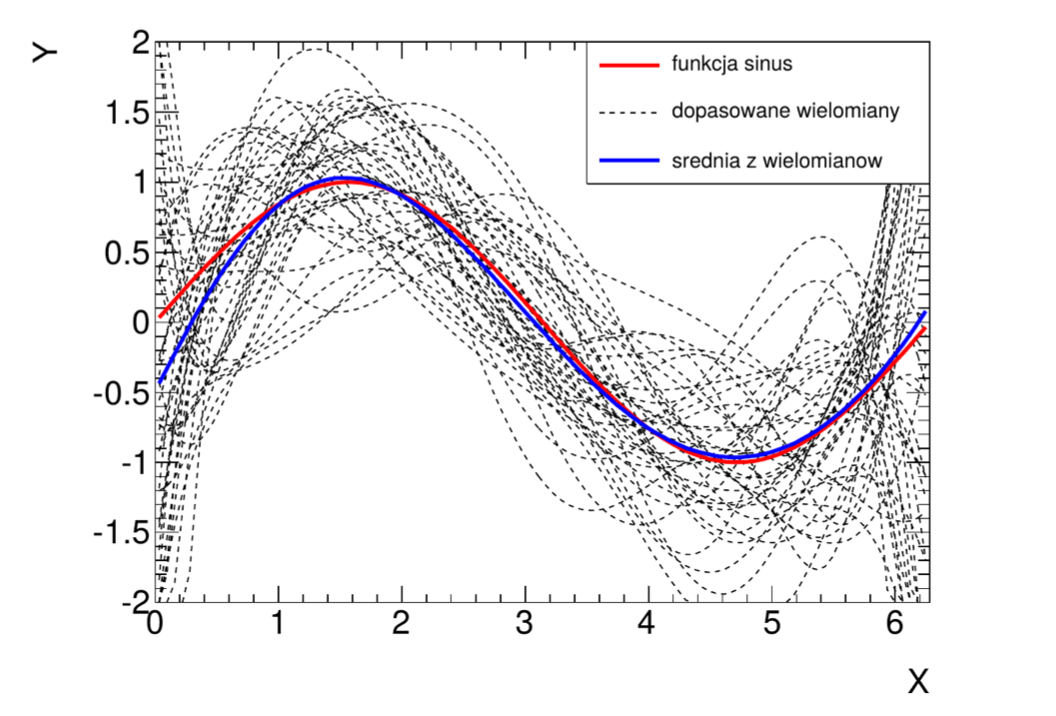
\includegraphics[scale=0.7]{res/avg1.png}
\caption[Caption for LOF]{Ilistracja działania \textit{ensemble learning} TODO:Podać źródło?\label{avg1}}
\end{figure} 

\subsubsection{Maszyna wektorów nośnych}
Maszyna wektorów wspierających (\textit{support vector machine, SVM}) jest modelem matematycznym, który~z~powodzeniem znajduje swoje zastosowaniu w~klasyfikacji oraz~regresji. Jej idea jest z~jednej strony dość prosta, natomiast z~drugiej sprawdza się w~dość skomplikowanych problemach\cite{svm1}. Na~rysunku \ref{svmIdea} przedstawiona został pomysł, który~kryje się za~tym algorytmem. Celem jego działania jest znalezienie hiperpłaszczyzny, która~dzieli dane wg klas w~optymalny sposób. W~tym celu, wybierana jest hiperpłaszczyzna, która~dzieli dane na~dwie klasy zachowując przy tym jak~największą odległość od~punktów obu tych klas\cite{svm2}. Podstawowa wersja tego algorytmu zapewnia tylko klasyfikacje binarną tzn. taką w~przypadku której~mamy tylko dwie klasy. W~celu rozszerzenia jego działania, istnieją dwa popularne podejścia  tj. \textit{one against one} oraz~\textit{one against all}\cite{svm3}. W~niniejszej pracy wykorzystane zostało pierwsze z~nich, które~polega na~stworzeniu maszyny wektorów wspierających dla każdej pary klas. Wynika z~tego, że~konieczne jest stworzenie $K(K-1)/2$ maszyn, gdzie ~$K$ oznacza liczbę atrybutów analizowanego zbioru danych. Ostatecznie, klasa dla konkretnego rekordu danych określana jest poprzez~,,głosowanie''. Ostatnią podstawową kwestią, którą należałoby wyjaśnić, jest pytanie jak~\textit{SVM} radzi sobie w~przypadku, gdy dane nie są separowalne liniowo, przy których jest również wielokrotnie wykorzystywana. W~takiej sytuacji wykorzystana jest transformacja danych, które~pozwala na~przedstawienie je w~przestrzeni o większej liczbie wymiarów. Rozwiązanie to zostało zilustrowane na rysunku \ref{svmKernel}. Algorytm dąży do~maksymalizacji odległości marginesu, który~powstaje podczas dobierania hiperpłaszczyzny (patrz rys. \ref{svmIdea}). W~wielu przypadkach nie jest możliwe dobranie takiej hiperpłaszczyzny, która~dokładnie podzieli dane. Rozwiązaniem w~tej sytuacji jest dodanie dodatkowego współczynnika $C$, który~dodatkowo uwzględniany jest w~procesie optymalizacji. Wartość $C$ stanowi o~tym jak~duży wpływ na~optymalizację błędu mają niepoprawnie sklasyfikowane przykłady w~procesie maksymalizacji marginesu i~jest jednym z~parametrów modelu, który~należy wyznaczyć w~celu otrzymania najbardziej optymalnego klasyfikatora. 

\begin{figure}[ht!]
\centering
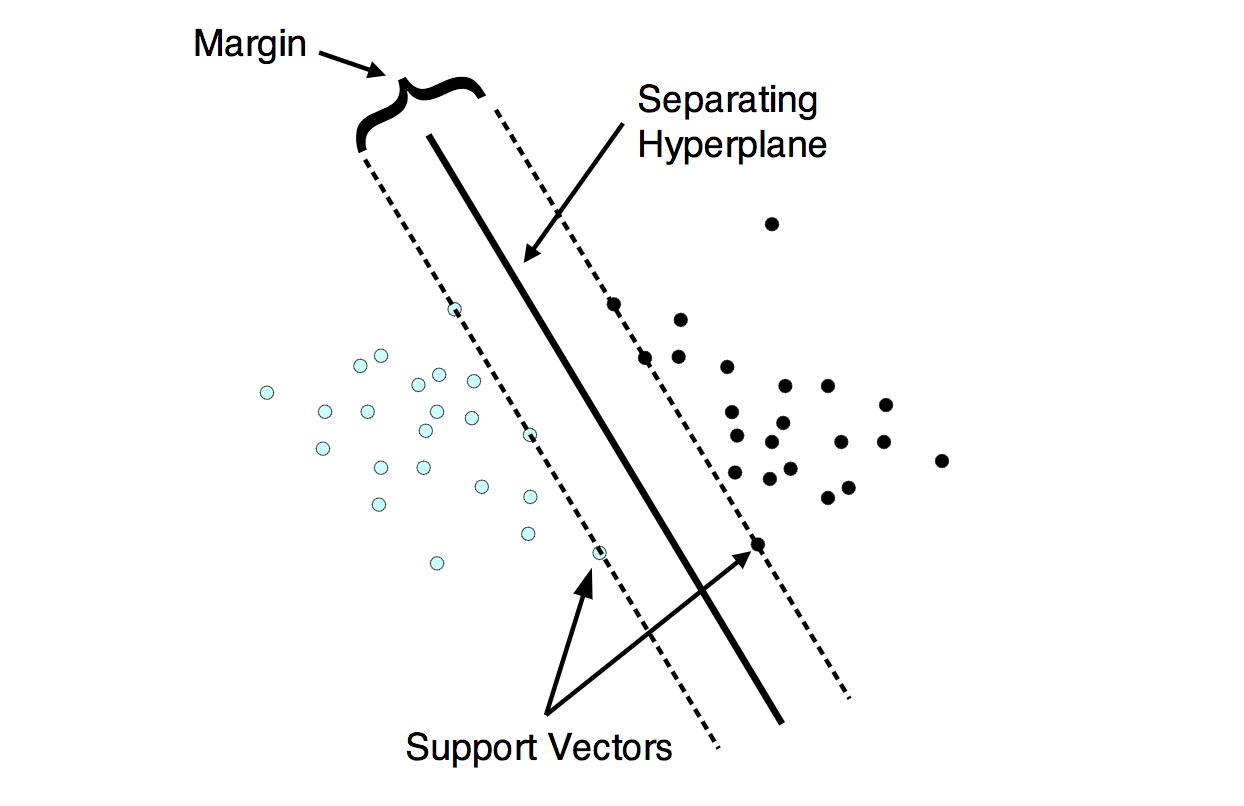
\includegraphics[scale=0.8]{res/svm1.png}
\caption[Caption for LOF]{Rysunek przedstawiający ideę maszyny wektorów wspierających. Źródło:\cite{svm2} \label{svmIdea}}
\end{figure} 

\begin{figure}[ht!]
\centering
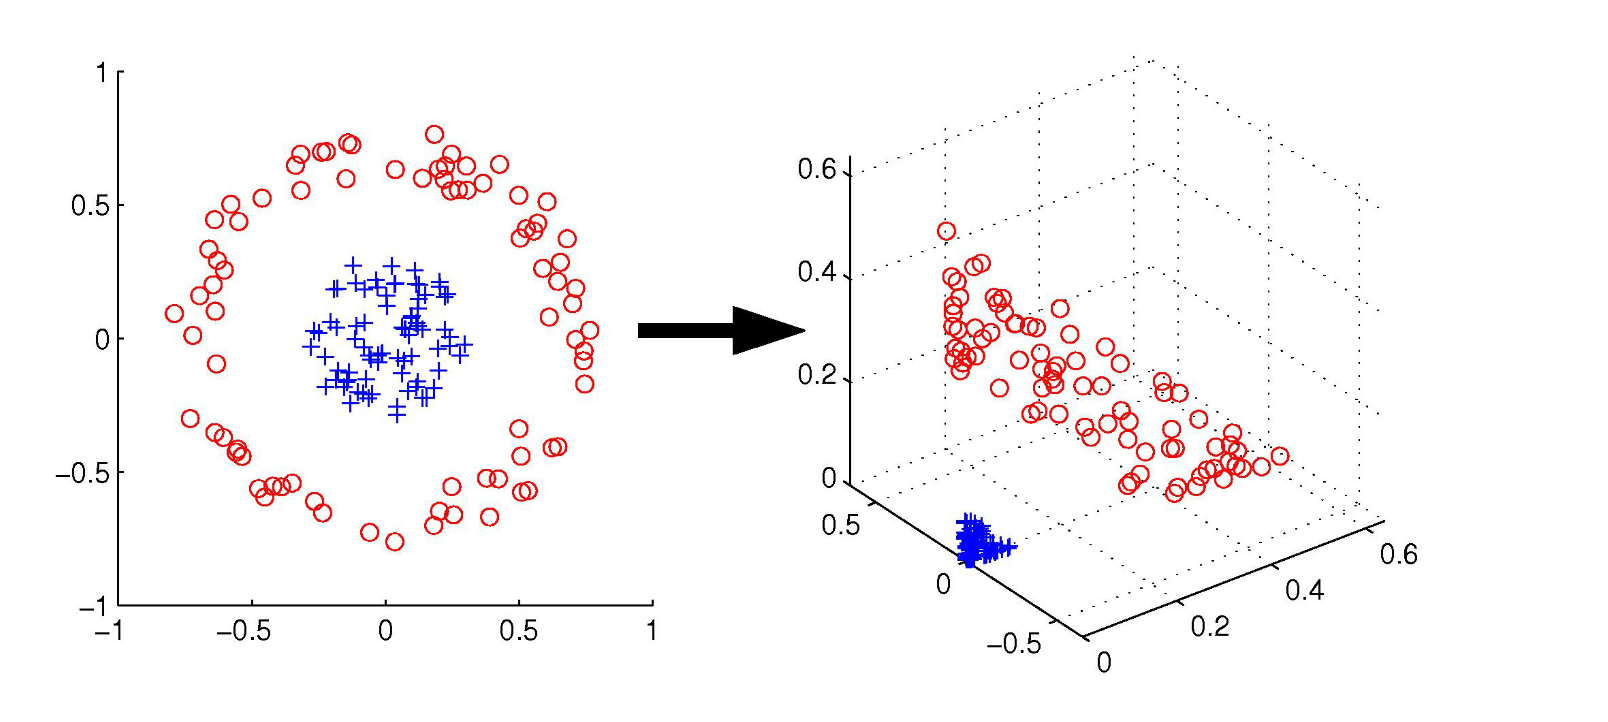
\includegraphics[scale=0.6]{res/svm2.png}
\caption[Caption for LOF]{Rysunek przedstawiający ideę transformowania danych do przestrzeni w której są one liniowo separowalne. Źródło:\cite{svmKernel} \label{svmKernel}}
\end{figure} 

\subsubsection{Tradycyjne sieci neuronowe}
% sieci neuronowe jako blackbox?
Niniejszy podrozdział powstał na~podstawie książki \cite{tadeusiewicz}. 
\noindent
Sztuczna sieć neuronowa, dalej nazywana siecią neuronową, jest metodę uczenia maszynowego, którego~inspiracją była biologia, a~konkretnie ludzki mózg i~występujące w~nim biologiczne sieci neuronowe. Podstawową odmianą sieci neuronowej jest sieć jednokierunkowa, czyli taka w~której nie występują sprzężenia zwrotne. Podstawową jednostką budulcową tego modelu jest neuron, który~przedstawiony został na~rysunku \ref{neuron}. Pojedynczy neuronu wykonuje operację sumy ważonej korzystając z~wartości na~swoich wejściach oraz~wagi przypisanej do~każdego wejścia. Wyjście z~kolei jest wynikiem zastosowania tzw. funkcji aktywacji na~wyniku uprzednio otrzymanym z~operacji sumy ważonej. Najpopularniejszymi funkcjami aktywacji w~tradycyjnych sieciach neuronowych są funkcja sigmoidalna, tangensoidalna oraz~,~zwłaszcza w sieciach konwolucyjnych opisanych w kolejnym rozdziale, funkcja ReLU (\textit{rectified linear activation function}. Funkcja ReLU wyraża się wzorem:
\begin{equation}
h=max(0,a),
\end{equation}
 przy czym $a=Wx+b$.
 
\begin{figure}[ht!]
\centering
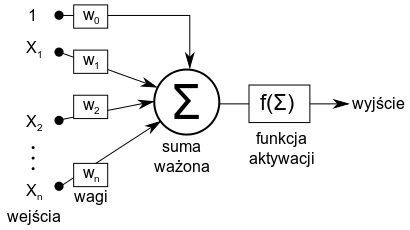
\includegraphics{res/neuron.png}
\caption[Caption for LOF]{Matematyczny model neuronu. Źródło:\url{http://pl.wikipedia.org/wiki/Plik:
Neuron_McCullocha-Pittsa.png}\label{neuron}}
\end{figure} 

\noindent
Cała sieć neuronowa jest niczym innym jak połączonymi ze~sobą neuronami. Każdemu połączeniu przypisana jest waga liczbowa, która~informuje o~tym jak~wpływają na~siebie poszczególne komórki sieci. Wszystkie neurony zgrupowaną są w~warstwy z~których możemy wyróżnić:
\begin{itemize}
\item warstwę wejściową,
\item jedną lub więcej warstw ukrytych,
\item warstwę wyjściową.
\end{itemize}

\noindent
W~każdej warstwie może znajdować się dowolna ilość neuronów. Przykład sieci neuronowej został przedstawiony na~rysunku \ref{net}.
\begin{figure}[ht!]
\centering
% obrazek pobrany z 
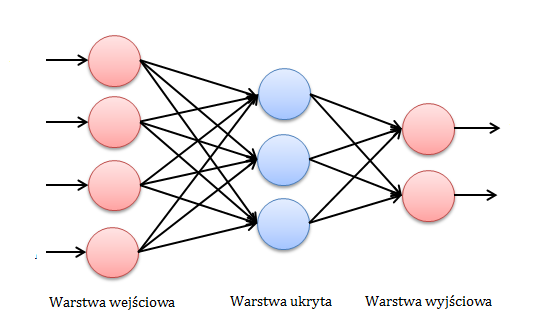
\includegraphics{res/exampleNet.png}
\caption[Caption for LOF]{Przykładowa jednokierunkowa sieć neuronowa. Źródło:\url{https://2ml4pa.bn1303.livefilestore.com/y2p6no6Dn0weHW3FG9tceTUS9lohx5ldcxvFZRhKdbeFQi2kntad_77gKeKIC-INcsFRCvGI-_DY9lMdZzaX8jkSHDvqlcT3qRnftpAt7esi4s/1.PNG?psid=1}\label{net}} 
\end{figure}
\noindent
W~każdej iteracji uczenia sieci, na~wejście podawany są dane. W~zależności o~odpowiedzi otrzymanej przez~sieć przeprowadzana jest poprawa wag. Po~przeprowadzeniu uczenia, sieć powinna ustalić wagi takie, aby~poprawnie odpowiadać na~kolejne sygnały wejściowe. W~ogólności mówimy o~minimalizacji błędu sieci $Q$ w~zależności od~wag sieci. W~równaniu aktualizującym wagi występuję również współczynnik $\eta$, który~jest tzw. współczynnikiem uczenia, który~zmniejsza wprowadzane poprawy wag sieci. Poprawka dla wagi konkretnego połączenia neuronowego z wagą $w_i$ definiujemy jako:
\begin{equation}\label{deltaRule}
\Delta w_i = - \eta \frac{\partial Q}{\partial w_i}.
\end{equation}
Dzięki temu współczynnikowi proces uczenia przebiega bardziej optymalnie. Jest on jednym z~parametrów modelu, który~należy wyznaczyć. Kolejnym z~parametrów tego modelu jest liczba neuronów w~warstwie ukrytej. Liczba neuronów w~warstwie wejściowej zależy od~liczby atrybutów naszych danych, natomiast wyjściowej od~tego na~ile kategorii dane są klasyfikowane. Pierwsze algorytmy uczenia, które~powstały potrafiły przeprowadzić uczenie sieci neuronowej tylko o~jednej warstwie. W~celu uczenia sieci wielowarstwowych powstał algorytm wstecznej propagacji. Błąd dla poszczególnych neuronów jest w~tym algorytmie obliczany ,,od przodu'' to znaczy zaczynając od~warstwy wyjściowej. Dla neuronów w~warstwie ukrytej błąd obliczany jako średnia ważona błędów neuronów do~których dany neuron wysłał swój sygnał. Sztuczne sieci neuronowe są często określane jako metoda typu czarnej skrzynki (\textit{black-box}). Po przeprowadzeniu uczenia, ciężko jest wyekstrahować wiedzę nabytą przez model i przedstawić ją w zrozumiały sposób, aczkolwiek jest to też tematem rozważanym przez naukowców \cite{blacboxann}. Jest to jeszcze bardziej utrudnione, ze względu na złożoność, w przypadku głębokich sieci neuronowych opisanych w kolejnym podrozdziale.

\subsubsection{Głębokie sieci neuronowe}\label{dnn}
Niniejszy rozdział zostal napisany na~podstawie pracy \cite{dnn1}.\\
% https://stats.stackexchange.com/questions/182734/what-is-the-difference-between-a-neural-network-and-a-deep-neural-network
% https://arxiv.org/pdf/1703.09039.pdf
Ideą stojącą za~głębokimi sieciami neuronowymi jest tworzenie sieci, które~posiadają wiele warstw ukrytych. Wiele, to znaczy od~kilku do~nawet kilku tysięcy. W~tradycyjnych sieciach neuronowych zazwyczaj występowało co najwyżej kilka warstw ukrytych, a~bardzo często tylko jedna. Udowodnione zostało, że~sieć o~jednej warstwie ukrytej posiadającej skończoną liczbę neuronów jest zdolna do~modelowania jakiejkolwiek funkcji pod~warunkiem występowania nieliniowych funkcji aktywacji w~neuronach \cite{anntheorem}, więc przez~długi okres czasu sieci o~większych rozmiarach nie były rozważane. W związku ze~wzrostem mocy obliczeniowej komputerów, a~także szerokim dostępie do~wszelkiego rodzaju danych nie jest jednak problemem stworzenie sieci o~wiele większych od~tradycyjnych. Okazało się, że~w~ten sposób otrzymane wyniki są znacznie lepsze i~sieci głębokie sieci stanowią kolejny przełom w~dziedzinie uczenia maszynowego. Dodatkowym aspektem, który umożliwia głębokim sieciom neuronowym osiąganie znacznie lepszych rezultatów jest inny sposób uczenia. TODO: napisac o tym uczeniu

Najłatwiej objaśnić działanie głębokich sieci neuronowych na~podstawie przykładu. W~przypadku tradycyjnych sieci neuronowych na~wejście sieci podawane są atrybuty, które~należy samemu określić. Są to wyznaczone matematycznie cechy w~zależności od~problemu. Przykładem takiej sytuacji możesz być rozpoznawanie konkretnych obiektów na~obrazie. Do~sieci neuronowej możemy podać w~takiej sytuacji konkretnie wyliczone cechy obrazu zamiast przekazywać wartość każdego piksela, co powodowałoby, że~sieć miałaby bardzo dużo wejść, a~co za~tym idzie, trudno byłoby ją nauczyć. Takimi cechami mogą być np. jasność obrazu, tekstura, wskaźnik występujących na~obrazie linii lub~okręgów oraz~wiele więcej. Przy operacji ekstrakcji cech z~obrazu następuję naturalnie pewna utrata informacji. W~przypadku głębokich sieci neuronowych nie dokonujemy ekstrakcji cech, co jest zasadniczą różnicą. Na~wejście sieci podawany są dane w~stanie ,,surowym''. Pozwala to na~uniknięcie utraty informacji, co przy odpowiedniej ilości danych oraz~dobrze zbudowanej sieci pozwala na~znacznie lepsze wyniki. Sieć podczas procesu uczenia jest w~stanie sama nauczyć się jakie cechy powinna rozpoznawać. Różnica ta została zilustrowana na~rysunku \ref{dnnDiff}.

\begin{figure}[ht!]
\centering
% obrazek pobrany z 
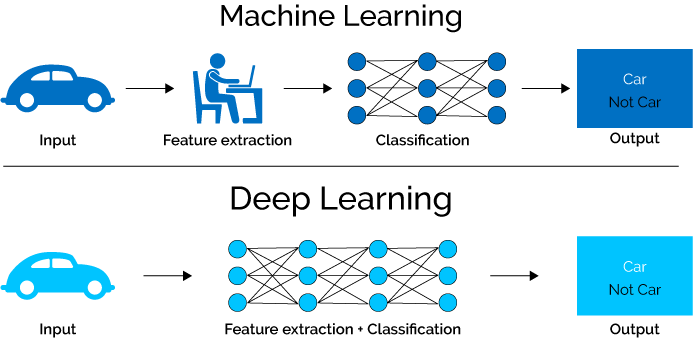
\includegraphics[scale=0.5]{res/dnn1.png}
\caption[Caption for LOF]{Różnica pomiędzy tradycyjnymi sieciami neuronowymi oraz głębokimi sieciami neuronowymi w kontekście ekstrakcji cech. Źródło: \url{https://hackernoon.com/log-analytics-with-deep-learning-and-machine-learning-20a1891ff70e}\label{dnnDiff}} 
\end{figure}

\subsubsection{Konwolucyjne sieci neuronowe}
Niniejszy rozdział został napisany na~podstawie\cite{nielsen}.\\
Konwolucyjne sieci neuronowe są najpopularniejszym typem głębokich sieci neuronowych. Znajdują swoje zastosowanie wszędzie, gdzie możemy zetknąć się z~potrzebą analizy obrazów. Ich nazwa wynika wynika z~faktu, iż~bazują one na~operacji konwolucji. W~przypadku tradycyjnych sieci neuronowych, w~sytuacji analizy obrazu bez ówczesnej ekstrakcji cech, należałoby podać na~każde wejście sieci wartość pojedynczego piksela. Problemem tego podejścia jest to, że~nie jest brana pod~uwagę przestrzenna natura obrazu. Każde wejście sieci traktowane jest indywidualnie i~nie jest ważne jego położenie na~obrazie.  Konwolucyjne sieci neuronowe wykorzystują przestrzenną naturę obrazu. Ich architektura jest do~tego dostosowana. Głównymi elementem sieci tego typu odróżniającymi je od~tradycyjnych jest istnienie warstw konwolucyjnej. W~przypadku tradycyjnych sieci neuronowych, zazwyczaj wyobrażamy sobie warstwę jako pojedyncza linie neuronów. Dla warstwy konwolucyjnej, bardziej naturalne jest jej przedstawienie w~dwóch wymiarach.
\begin{figure}[ht!]
\centering
% obrazek pobrany z 
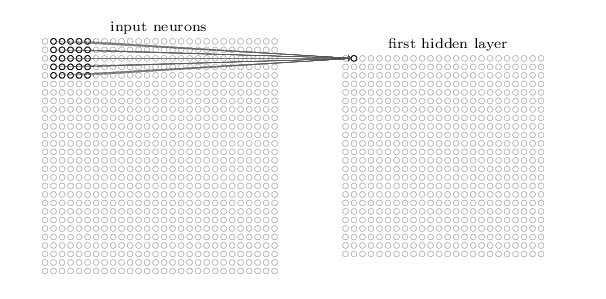
\includegraphics[scale=0.6]{res/cnn1.png}
\caption[Caption for LOF]{Warstwa wejściowa konwolucyjnej sieci neuronowej przedstawiona w dwóch wymiarach. Źródło:\cite{nielsen}\label{cnn1}} 
\end{figure}

\noindent
Wartością każdego neuronu wejściowego jest wynik operacji konwolucji. W~celu otrzymania wszystkich wejść należy ,,przesuwać'' maskę po~całym obrazie. W~zależności od~rozmiaru maski (zazwyczaj 3x3, 5x5 lub~7x7) otrzymujemy odpowiednią liczbę wejść sieci. Operacja ta została przedstawiona na~rysunku \ref{cnn1}. Należy wspomnieć, że~wagi wszystkich neuronów są wspólne. Można stwierdzić, że~w~ten sposób pierwsza warstwa służy do~wykrycia dokładnie jednej cechy obrazu. Jedna cecha na~jedną warstwę, to byłoby jednak za~mało, więc ostatecznie najlepiej przedstawić pojedyncza warstwę konwolucyjną w~trzech wymiarach, co można zobaczyć na~rysunku \ref{cnn2}.
\begin{figure}[ht!]
\centering
% obrazek pobrany z 
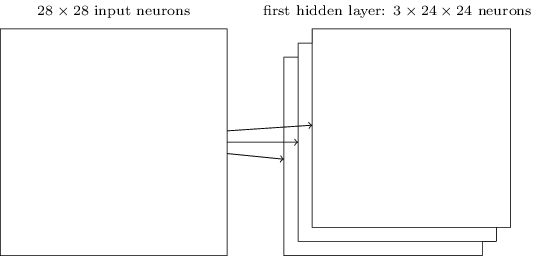
\includegraphics[scale=0.6]{res/cnn2.png}
\caption[Caption for LOF]{Warstwa wejściowa konwolucyjnej sieci neuronowej przedstawiona w trzech wymiarach. Źródło:\cite{nielsen}\label{cnn2}} 
\end{figure}
\noindent
W~sieciach konwolucyjnych, oprócz warstw konwolucyjnych, występują także warstwy typu \textit{pooling}, które~pozwalają na~pomniejszenie obrazu, co z~kolei redukuje w~pewnym stopniu koszty związane z~obliczeniami. Jedną z~podstawowych wykorzystywanych technik jest tzw. \textit{max-pooling}. Ponownie używając maski dowolnego rozmiaru (zazwyczaj 2x2) ,,przechodzimy'' po~całym obrazie, lecz tym razem wybierając do~warstwy po~operacji \textit{poolingu} piksel o~najwyższej wartości.
\begin{figure}[ht!]
\centering
% obrazek pobrany z 
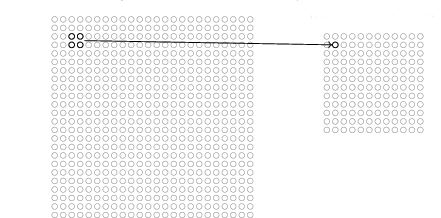
\includegraphics[scale=0.6]{res/pooling.png}
\caption[Caption for LOF]{Warstwa typu \textit{pooling}. Źródło:\cite{nielsen}\label{pooling}} 
\end{figure}
\noindent
Po~warstwach konwolucyjnych oraz~typu \textit{pooling}, których ilość jest arbitralna, następuje przejście do~warstw w pełni połączonych (\textit{fully connected}) znanych z tradycyjnych sieci neuronowych, gdzie dokonywana jest ostateczna klasyfikacja. Kompletna architektura sieci konwolucyjnej została przedstawiona została na~rysunku \ref{cnn3}.

\begin{figure}[ht!]
\centering
% obrazek pobrany z https://www.kernix.com/blog/a-toy-convolutional-neural-network-for-image-classification-with-keras_p14
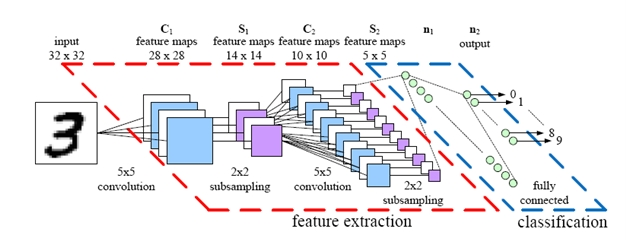
\includegraphics[scale=0.75]{res/cnn3.jpg}
\caption[Caption for LOF]{Architektura konwolucyjnych sieci neuronowych. Źródło: \url{ https://www.kernix.com/blog/a-toy-convolutional-neural-network-for-image-classification-with-keras_p14}\label{cnn3}} 
\end{figure}


\subsection{Przeuczenie}\label{overfitting_section}
Przeuczenie (\textit{overfitting}) jest jednym z~głównych problemów na~który można napotkać podczas korzystania z~algorytmów uczenia maszynowego. W~pierwszym zetknięciu z~uczeniem maszynowym mogłoby się wydawać, że~im mniejszy błąd uzyskany podczas uczenia, tym lepiej. Okazuje się jednak, że~podczas uczenia, zwłaszcza gdy model posiada zbyt wysoką liczbę stopni swobody, algorytm dopasowuje się ściśle do~konkretnych danych, które~w~rzeczywistości są w~pewnym stopniu zaszumione. Można powiedzieć, że~algorytm ,,uczy się'' wtedy na~pamięć, co nie jest oczekiwanym rezultatem, ponieważ~staje się on wtedy również mniej skuteczny dla danych innych niż uczące.  Model jest wtedy niezdolny do~generalizacji, a~właśnie po~to został stworzony, aby~można było do~użyć na~danych, których wcześniej ,,nie widział''. Analogicznie, można spotkać się też z~problemem niedouczenia \textit{underfitting}. Oznacza to, że~funkcja, którą chcemy modelować jest zbyt skomplikowana dla naszego modelu, co wynika z~tego, że~posiada on zbyt niską liczbę stopni swobody. Obie sytuacje zostały przedstawione na~rysunku \ref{overfitting}.

\begin{figure}[ht!]
\centering
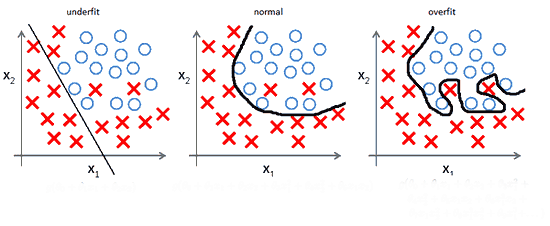
\includegraphics[scale=0.8]{res/overfitting.png}
\caption[Caption for LOF]{Problem przeuczenia oraz niedouczenia na przykładzie klasyfikacji. Źródło:\url{http://mlwiki.org/index.php/Overfitting}\label{overfitting}} 
\end{figure}

\subsection{Tablica pomyłek i krzywa ROC}
% Please add the following required packages to your document preamble:
% \usepackage{multirow}
% \usepackage[table,xcdraw]{xcolor}
% If you use beamer only pass "xcolor=table" option, i.e. \documentclass[xcolor=table]{beamer}
\begin{table}[]
\centering

\begin{tabular}{llllll}
                                                         &                                                              & \multicolumn{2}{c}{klasa rzeczywista}                                                                                                                                    &  &  \\ \cline{3-4}
                                                         & \multicolumn{1}{l|}{}                                        & \multicolumn{1}{l|}{\cellcolor[HTML]{9B9B9B}{\color[HTML]{000000} klasa pozytywna}} & \multicolumn{1}{l|}{\cellcolor[HTML]{9B9B9B}{\color[HTML]{000000} klasa negatywna}} &  &  \\ \cline{2-4}
\multicolumn{1}{c|}{}                                    & \multicolumn{1}{l|}{\cellcolor[HTML]{9B9B9B}klasa pozytywna} & \multicolumn{1}{l|}{prawdziwie pozytywna}                                           & \multicolumn{1}{l|}{fałszywie pozytywna}                                            &  &  \\ \cline{2-4}
\multicolumn{1}{c|}{\multirow{-2}{*}{klasa predykowana}} & \multicolumn{1}{l|}{\cellcolor[HTML]{9B9B9B}klasa negatywna} & \multicolumn{1}{l|}{fałszywie negatywna}                                            & \multicolumn{1}{l|}{prawdziwie negatywna}                                           &  &  \\ \cline{2-4}
                                                         &                                                              &                                                                                     &                                                                                     &  & 
\end{tabular}
\caption{Tablica pomyłek} \label{table:confusionmatrix}
\end{table}
Tablica pomyłek może posłużyć do~oceny jakości klasyfikacji binarnej. Rozważając taką klasyfikację, model może odpowiedzieć tylko na~dwa sposoby: pozytywnie oraz~negatywnie. Odpowiedź może być błędna lub~poprawna, co daje cztery możliwości. Na~tej podstawie otrzymujemy cztery wielkości:
\begin{itemize}
\item ilość predykcji prawdziwie pozytywnych (\textit{true positive}, TP),
\item ilość predykcji fałszywie negatywnych (\textit{false negative}, FN),
\item ilość predykcji fałszywie pozytywna (\textit{false positive}, FP),
\item ilość predykcji prawdziwie negatywnych (\textit{true negative}, TN).
\end{itemize}

\noindent
Powyższe możliwości zostały zestawione w~tabeli \ref{table:confusionmatrix}. Idąc dalej możemy określić TPR(\textit{true positive rate}) oraz~FPR(\textit{false positive rate}):


\begin{equation}
TPR = \frac{TP}{P} = \frac{TP}{TP+FN} 
\end{equation}
\noindent
oraz

\begin{equation}
FPR = \frac{FP}{N} = \frac{FP}{FP+TN},
\end{equation}

przy czym $T$ oraz~$N$ oznaczają kolejno wszystkie próbki pozytywne oraz~wszystkie próbki negatywne. Na~podstawie $TPR$ oraz~$FPR$ z~kolei istnieje możliwość wykreślenia krzywej ROC(\textit{Receiver Operating Characteristic}). W~celu wykreślenia krzywej ROC stworzony model powinien na~wyjściu zwracać prawdopodobieństwo  przynależności do~jednej z~dwóch klas. W~zależności od~ustalenia punktu odcięcia tj. wartości prawdopodobieństwa dla którego~stwierdzamy przynależność do~danej klasy otrzymujemy dwie wartości TPR oraz~FPR dla danego punktu odcięcia. Ostatecznie można określić krzywą ROC jako funkcję zależną od~punktu odcięcia, która~została przedstawiona na~rysunku \label{roc}. W~celu opisania jakości klasyfikatora jedną liczbą można posłużyć się także polem powierzchni pod~krzywą ROC.

\begin{figure}[ht!]
\centering
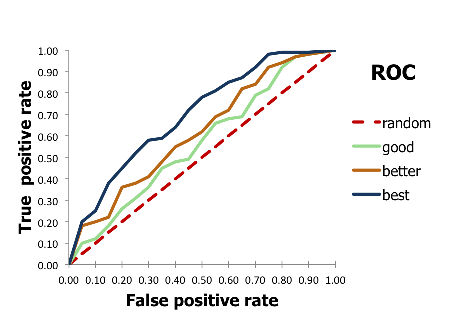
\includegraphics[scale=0.7]{res/roc3.png}
\caption[Caption for LOF]{Krzywa ROC. Źródło:\url{http://scikit-learn.org/stable/_images/sphx_glr_plot_roc_001.png}\label{roc}} 
\end{figure}



\subsection{Problemy wynikające z małej ilości danych}\label{problems}
W~przypadku uczenia maszynowego z~nauczycielem istnieje potrzeba posiadania danych, które~posłużą do~uczenia. Im więcej danych, tym szerszy wachlarz metod, których możemy użyć. Tak jak~zostało jednak wspominane w~rozdziale \ref{matter}, istnieją wciąż dziedziny w~których może się okazać, że~nie znajdujemy się w~tej komfortowej sytuacji dysponowania milionami rekordów danych. W~takich okolicznościach spotkać się możemy z~następującymi problemami:

\begin{itemize}
\item przeuczenie staję się bardzo dużym problemem i jest trudniejsze do uniknięcia,
\item elementy odosobnione mają dużo większy wpływ na proces uczenie,
\item szum w danych ma również większy wpływ na wyniki działania algorytmów uczenia maszynowego.
\end{itemize}
Istnieje jednak kilka sposobów, które~pomagają radzić sobie w~sytuacji niskiej ilości danych, aczkolwiek należy pamiętać, że~nie sprawią, że~wykorzystanie uczenia maszynowego stanie się możliwe jeśli danych jest rzeczywiście za~mało. Nie da się także jednoznacznie określić, gdzie znajduje się granica, która~mówi o~tym czy~ilość danych jest niewystarczająca. Zależy to od~konkretnego przypadku. Istnieje kilka metod optymalizacji w~przypadku niskiej ilości danych:
\begin{itemize}
\item użycie nieskomplikowanych modeli, co przeciwdziała problemowi przeuczenia,
\item użycie metod walidacji krzyżowej zamiast tradycyjnego podejścia podziału danych na zbiór uczący oraz testowy,
\item ekstrakcja lub redukcja cech
\item regularyzacja,
\item sztuczne powielanie danych poprzez wykorzystanie ich symetrii (np. w obrazach obrócenie w poziomie lub w pionie itp.).
\end{itemize}


\subsection{Wykorzystane metody optymalizacji}
Niniejszy podrozdział zawiera opis metod, które~zostały użyte w~tej pracy w~celu optymalizacji uczenia maszynowego. Wyniki 
natomiast, przedstawione zostały w~rozdziale \ref{results}.
\subsubsection{Sztuczne powiększenie zbioru danych}
Sztuczne powiększenie zbioru (\textit{data augmentation}) danych w~przypadku danych graficznych jest najłatwiejszą oraz~najpopularniejszą metodą, która~służy do~minimalizowania efektu przeuczenia\cite{dataaugment}. Polega ona na~transformacji danych tj. obrazów, przy zachowaniu ich kategorii. Często przekształcenia te związane są z~symetrią obrazu, lecz nie tylko. Wymienić można między innymi:
\begin{itemize}
\item odbicie lustrzane obrazu (w pionie lub w poziomie),
\item rotacja obrazu o dany kąt,
\item przybliżenie obrazu,
\item przeskalowanie,
\item przycięcie obrazu.
\end{itemize}
Algorytm uczony na w ten sposób wygenerowanych obrazach cechuje się mniejszą podatnością na efekt przeuczenia. 
\subsubsection{Walidacja krzyżowa}
We wszystkich algorytmach uczenia maszynowego występują parametry, które~należy określić dla danego modelu predykcyjnego. W~zależności od~metody, oznaczają co innego, ale~w~każdym przypadku ważny jest optymalny ich dobór, aby~uzyskać jak~najlepszy wynik.W najbardziej podstawowym przypadku, zbiór danych, który~posiadamy, dzielimy na~dwie części tj. zbiór uczący oraz~testowy. Pierwszy z~nich służy do~uczenia, a~drugi do~określanie jakości stworzonego modelu. W~przypadku przeszukiwania przestrzeni parametrów modelu w~celu ich optymalnego doboru, kierujemy się wynikiem predykcji dla zbioru testowego. Jest to naturalne ze~względu na~występujący efekt przeuczenia dla danych uczących. Ocena na~wcześniej ,,niewidzianych'' przez~model danych będzie bardziej obiektywna. Przy takim rozwiązaniu jednak, pewna część informacji ze~zbioru testowego również ,,wycieka'' do~naszego modelu, więc jest to również metodologicznie błędne podejście. Idealnym rozwiązaniem było podzielenie naszych danych na~zbiór uczący, testowy oraz~walidujący. Zbiór walidujący posłużyłby wtedy do~doboru optymalnych parametrów modelu, a~następnie zbiór testowym do~ostatecznej ewaluacji. Łatwo jednak wywnioskować, że~w~sytuacji, gdy ilość danych jest niska, tworzenie trzech osobnych zbiorów jest mało optymalnym rozwiązaniem, ponieważ~jeszcze mniej danych wykorzystane zostanie do~uczenia modelu. Rozwiązaniem tego problemu jest walidacjia krzyżowa (\textit{cross validation}). W~tej metodzie dzielimy zbiór który~posiadamy na~$k$ losowych części, a~następnie uczymy oraz~testujemy model $k$ razy przy czym za~każdym razem do~uczenia wykorzystujemy $k-1$ części danych, a~do testowania jedną część, która~nie została użyta do~uczenia modelu. Jako ostateczny wynik ewaluacji przyjmujemy średnią z~$k$ otrzymanych wyników. Korzystając z~tej metody, parametry modelu zostaną dobrane używając większej ilości danych minimalizując efekt przeuczenia. Takie podejście z~pewnością powoduje znacznie większe zapotrzebowanie na~zasoby obliczeniowe. W~skrajnym przypadku, gdy $k=N$, przy czym $N$ oznacza liczbę wszystkich rekordów, mówimy o~metodzie \textit{leave one out}. W~praktyce jednak, stosuję się walidację krzyżową przy $k=10$, co jednak wciąż generuje bardzo dużo obliczeń. Graficzna ilustracja tej metody została przedstawiona na~rysunku \ref{cv}.
\begin{figure}[ht!]
\centering
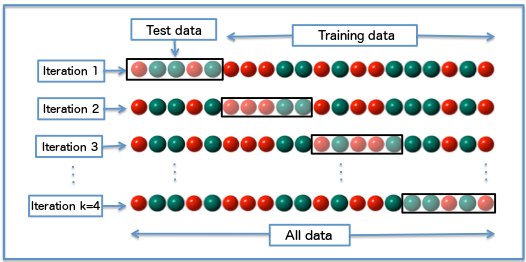
\includegraphics[scale=0.7]{res/cv.jpg}
\caption[Caption for LOF]{Przykład walidacji krzyżowej. Źródło: \url{https://upload.wikimedia.org/wikipedia/commons/1/1c/K-fold_cross_validation_EN.jpg}} \label{cv} 
\end{figure}


\subsubsection{Ekstrakcja cech}
Ekstrakcja cech jest nieodwracalną operacją na~danych, które~posiadamy. Polega ona na~transformacji atrybutów w~taki sposób, aby~zmniejszyć ich liczbę. Zawsze wiąże się to z~utratą informacji, ponieważ~nie jest możliwe reprezentacja tej samej informacji przy zmniejszonej wymiarowości danych pomijając sytuację, gdy atrybuty są od~siebie zależne. Zmniejszanie wymiarowości danych przez~eliminacje redundantnych atrybutów nazywamy z~kolei redukcją cech. 
Ekstrakcja cech dokonywana jest zazwyczaj w~sytuacji, gdy ilość atrybutów danych jest zbyt duża w~stosunku do~ilości danych, które~posiadamy lub~atrybuty są zbyt niskiego poziomu, aby~dana metoda uczenia maszynowego była w~stanie modelować funkcję atrybutów. Druga przyczyna jednak zależy od~użytej metody, ponieważ~w~przypadku głębokich sieci neuronowych, pod~warunkiem dobrania odpowiednich parametrów oraz~architektury sieci, możemy spodziewać się lepszych wyników dla atrybutów niższego poziomu (przed zastosowaniem ekstrakcji cech) jak~zostało to opisane w~rozdziale \ref{dnn}. Można wyróżnić dwa podejścia do~ekstrakcji cech. Jedno przy wykorzystaniu metod matematycznych np. PCA lub~LDA, które zostały opisane poniżej. O~drugim podejściu mówimy natomiast w~sytuacji, gdy transformacja danych dokonywana jest przy użyciu dodatkowej wiedzy, którą posiadamy na~temat danych. Na~przykładzie obrazów możemy powiedzieć, że~uzyskanie z~nich informacji opisujących ich konkretne parametry mówiące nam np. o~krawędziach na~obrazie czy~istnieniu na~nim linii lub~okręgów, jest ekstrakcją cech. W~przypadku z~kolei dźwięku, cechami niskiego poziomu, można nazwać amplitudę w~funkcji czasu, natomiast cechą wysokiego poziomu np. wskaźnik zmiany znaku amplitudy.
\paragraph{PCA}\mbox{}\\
Analiza głównych składowych (\textit{principal component analysis}, PCA) jest metodą, która~jest z~powodzeniem wykorzystywana do~ekstrakcji cech. Jej działanie polega na~otrzymaniu kolejnych głównych składowych o~największej wariancji. W~praktyce można wyobrazić sobie, że~operacja ta obraca układ współrzędnych w~ten sposób, aby~zmaksymalizować wariancję. Każdy kolejna składowa powinna być ortogonalna do~poprzedniej w~celu utrzymania jak~największej niezależności zmiennych. Operacja została dla przypadku dwuwymiarowego została przedstawiona na~rysunku \ref{pca}. W~celu ekstrakcji cech, w~nowej przestrzeni brane pod~uwagę jest tylko arbitralnie dobrana liczba nowych atrybutów.
\begin{figure}[ht!]
\centering
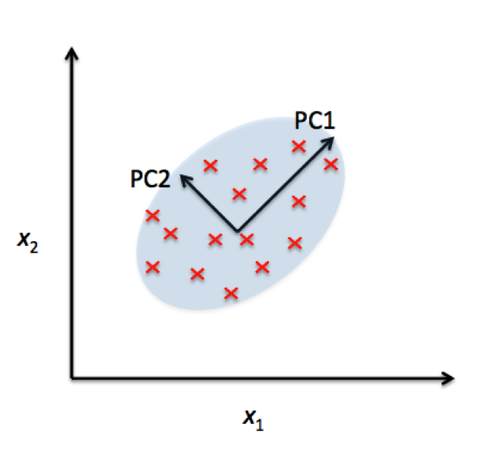
\includegraphics[scale=0.5]{res/pca.png}
\caption[Caption for LOF]{Graficzna ilustracja analizy głównych składowych. Źródło:\url{https://sebastianraschka.com/faq/docs/lda-vs-pca.html}} \label{pca} 
\end{figure}

\paragraph{LDA}\mbox{}\\
Liniowa analiza dyskryminacyjna (\textit{linear discrimant analysis, LDA}) jest metodą, która~działa w~podobny sposób do~PCA. Również w~tej metodzie na~celu mamy znalezienie nowego układu współrzędnych dla naszych danych. Różnica jednak polega na~tym, że~zamiast maksymalizować wariancję, maksymalizujemy separowalność kategorii rzutując dane na~konkretną oś. Można wywnioskować również w~takim razie, że~w~przeciwieństwie do~PCA, w~tej metodzie pod~uwagę są również klasy konkretnych rekordów. Operacja została zilustrowana na~rysunku \ref{lda}. 

\begin{figure}[ht!]
\centering
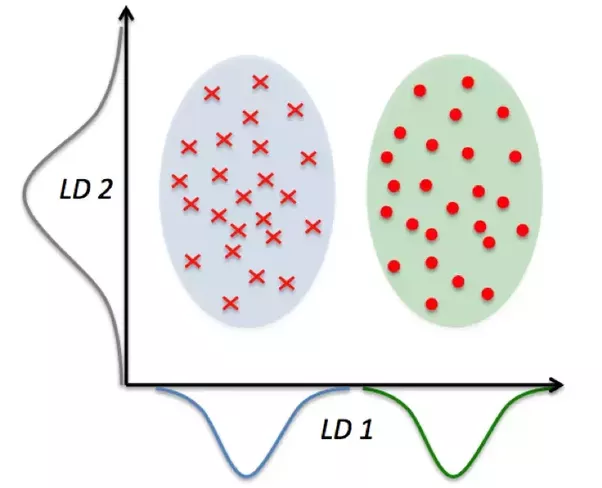
\includegraphics[scale=0.5]{res/lda.png}
\caption[Caption for LOF]{Graficzna ilustracja liniowej analizy dyskryminacyjna. Źródło:\url{https://qph.ec.quoracdn.net/main-qimg-daf30ce6ecf85035af12e97659108f0a}} \label{lda} 
\end{figure}
